\section{Vision based navigation system}
Since camera is the only sensor our robot have for detecting object on the field, various image processing algorithm will be used to identify many type of objects on the field. Currently balls, field lines and field boundary can be detected as describe below. The position of objects in three dimensional coordinate can be determined from an image according to a principle of a pinhole camera model. Moreover, information outside of the soccer field can be used as addition landmarks for determining the direction toward the opponent goal. We found a method which has a potential for detecting objects around the soccer field which can be used as a landmark. However, this method is still at the experimental stage at the moment. 

	\subsection{Position Determination}
	\label{threeToTwo}
	Three dimensional position of an object $(x,y,z)$ can be estimated when the object is identified in an image. The necessary information consists of a selected pixel on image coordinate $(u,v)$ that belong to the object, forward kinematic from a robot base to a camera and camera's properties. Any objects on the world can be projected on image plane via perspective transform as described in equation \ref{pinHoleCamEq}. We can also project object on image plane into another plane (in our case, ground is the projected plane) which gives us a three dimensional coordinate respect to camera. Coordinate of objects in robot frame can be obtained by transforming camera coordinate to robot coordinate using forward kinematic.
	\begin{equation}
		\label{pinHoleCamEq}
		\frac{1}{w}
		\begin{bmatrix}
		u \\
		v \\
		1 
		\end{bmatrix} =
		\begin{bmatrix}
			f_{x}	&	0	&	0\\
			0		&	f_{y} & 0\\
			0		&	0	&	1\\	
		\end{bmatrix}
		\begin{bmatrix}
			x \\
			y \\
			z \\
		\end{bmatrix}
	\end{equation}
	
	\subsection{Color Segmentation}
	\label{colorSeg}
	Each pixels in an image will be classified into eight colors (green, black, orange, blue, yellow, magenta, cyan and white). We use HSV color space for classifying color of each pixel based on their value. Then, the watershed segmentation is applied to get a better result on color segmentation.
	\begin{figure}[H]
		\begin{subfigure}{.5\textwidth}
			\centering
			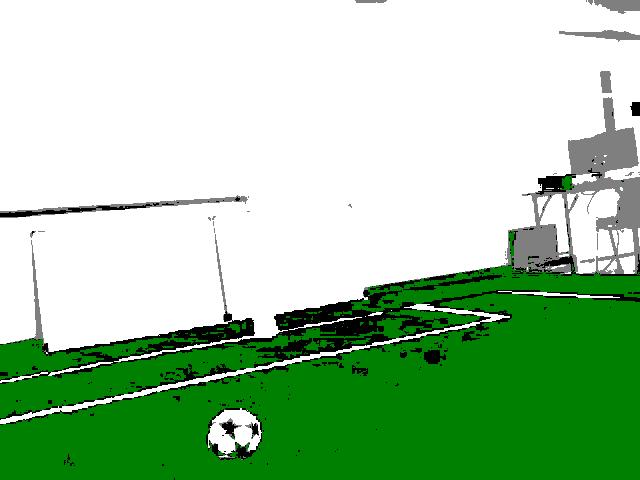
\includegraphics[width=\textwidth]{image/colormap.png}
			\caption{a). without watershed.}
			\label{fig:sfig1}
		\end{subfigure}%
		\begin{subfigure}{.5\textwidth}
			\centering
			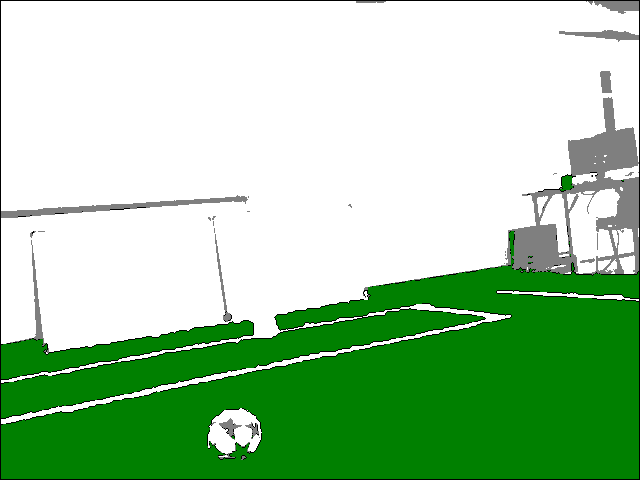
\includegraphics[width=\textwidth]{image/colormap_watershed.png}
			\caption{b) with watershed.}
			\label{fig:sfig2}
		\end{subfigure}
		\caption{color segmentation (black color represent unknown region, gray color represent black region)}
		\label{fig:fig}
	\end{figure}
	
	\subsection{Field Boundary Detection}
	An information about field boundary is important for our soccer robot. This information can be used later on other image processing algorithm. We detect a field boundary by scanning an image from top to bottom and find a first green pixel for each columns of an image. Then, apply median filter to filter out some noise. We also detect an outliers by cut out points which has the position on y axis higher than 1.5 of standard deviation. 
	\begin{figure}[H]
		\centering
		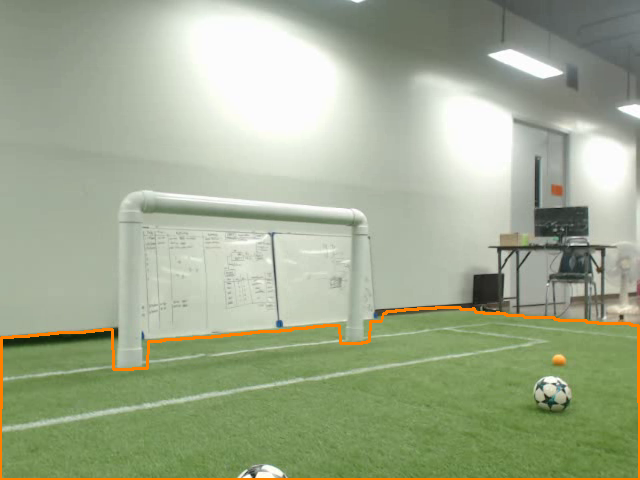
\includegraphics[width=0.6\textwidth]{image/fieldLine1.png}
		\caption{Example of field boundary detection}
		\label{fieldBoundary}
	\end{figure}
	
	\subsection{Ball Detection}
	From the competition in Robocup asia pacific 2017 we have tried using HAAR feature for ball detection. A lot of false positive detections have occurred, so we have to remove the un-related background by ignoring all objects outside a field boundary. The approach for ball detection has been slightly changed as followed.
	\begin{enumerate}
		\item As the ball contains white component mostly, the white color segmentation from \ref{colorSeg} has been used. Ramer---Douglas---Peucker algorithm was used to classify how well the circle shape the object is. And then the region of the interests (ROI) of the detected objects would be used for consideration.
		
		\item The ROI(s) from previous step were checked with well-trained HAAR cascade classifier (using adaboost).  Because we have limited the ROI(s), the scanning is faster than before. 
	\end{enumerate}
	
	\begin{figure}[H]
		\centering
		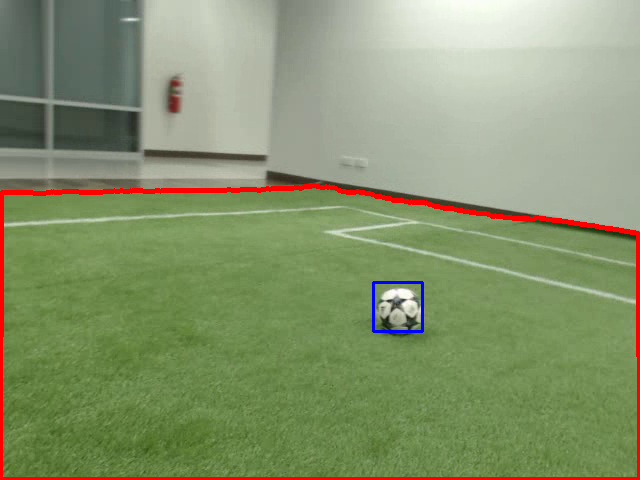
\includegraphics[width=0.6\textwidth]{image/ballDetection.png}
		\caption{Example of ball detection}
		\label{ball}
	\end{figure}
	
	\subsection{Line Detection}
	Line information should be useful for localization in future work. To detecting a line, we scan an image inside a field boundary from top to bottom every 40 image columns and find points where color is changes from green to white. Three dimensional coordinate of those point can be obtained as we mention in \ref{threeToTwo}. Those points on a field line can be treated like a point cloud from laser scanner and be used by a particle filter.
	\begin{figure}[H]
		\centering
		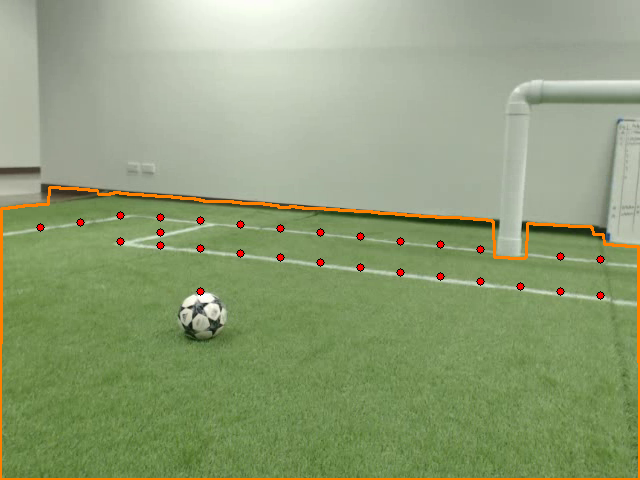
\includegraphics[width=0.6\textwidth]{image/lineDetection.png}
		\caption{Example of line detection}
		\label{lineDetection}
	\end{figure}
	\subsection{Landmark Detection}
%	ในการตำแหน่งของหุ่นยนต์ในสนามที่สมมาตรทั้งสองข้างนั้นในบางครั้งในการคำนวณตำแหน่งของหุ่นยนต์โดยกำหนดตัวแปรตั้งต้นแค่ครั้งแรกในการเริ่มเกมด้วยปัจจัยหลายๆอย่างเช่น การล้มของหุ่นยนต์ อาจทำให้อัลกอริทึ่มประมาณค่าตำแหน่งผิดพลาดได้เนื่องการจากหลงทิศทาง ดังนั้นเราจึงเสนอวิธีการ detect หา landmark ที่อยู่รอบๆสนามเพื่อเป็นสิ่งที่ช่วยในการยืนยันทิศทางที่ถูกต้องแก่ตัวหุ่นยนต์ได้
	From a new rule of Robocup humanoid soccer robot, there is no explicit landmark on the field to indicate direction toward our own goal or the opponent goal. We wonder if any landmark outside a field can be detected by a robot inside the field. These landmarks will be an important information for a robot to recognize a direction of itself.
	\paragraph{}
%	วิธีการ detect landmark นั้นเราใช้วิธีการ deep learning อัลกอริทึ่มที่มีชื่อว่า Fully-convolution Siamese network ถูกนำเสนอใน \ref{paperSiameseFC} ซึ่งวิธีการนี้ถูกใช้สำหรับการ track วัตถุที่มีการเคลื่อนที่โดยพลการ(arbitrary object tracking) และสามารถ track วัตถุที่ไม่เคยเห็นมาก่อนได้ โดยอินพุตของโมเดลนี้จะมี exemplar image จากเฟรมแรก และ Search image จากเฟรมต่อไปซึ่งจะถูก initial ในเฟรมแรกของวิดีโอและโมเดลจะทำการทำนายตำแหน่งของวัตถุที่ถูกต้องในเฟรมต่อไปได้โดยโมเดลจะให้เอาท์พุตออกมาเป็น score map ซึ่งจะบอกถึงความน่าจะเป็นของตำแหน่งที่ถูกต้องของวัตถุใน Search image ได้
	Fully-Convolution Siamese Network is a kind of neural network which capable to track an arbitrary object. This algorithm was proposed in \cite{DBLP:journals/corr/BertinettoVHVT16}. This network will look at example image of an object once and capable of tracking that object for an entire image sequence. We can tweak tracking algorithm and also some network architecture to make it more suitable for our problem. At this state, this concept of our landmark detection is still an experimental. Further work will be done to prove that this algorithm can be available for our robot. 
%	\paragraph{}
%	เราทำการประยุกต์ใช้โมเดลนี้โดยการใช้ exemplar image เป็นภาพของวัตถุที่เราให้เป็น landmark และใช้ Search image เป็นภาพทั้งภาพในทุกๆเฟรมของวิดีโอโดยปกติแล้ว score map ที่ได้จากโมเดลนี้จะมีค่าความน่าจะเป็นของจุดที่คิดว่าเป็นตำแหน่งที่ถูกต้องของวัตถุสุงอยู่ค่าหนึ่งและเมื่อไม่พบวัตถุที่มีความเหมือนกับ exemplar image ค่าที่สุงที่สุดของ score map จะมีค่าน้อยเราจึงทำการใช้ค่า threshold เป็น filter เพื่อบ่งบอกว่ามีวัตถุที่เป็น landmark อยู่ในภาพหรือไม่และด้วยวิธีการเดียวกันนี้ทำให้เราสามารถ detect เสาของ goal เพื่อช่วยให้การหาตำแหน่งgoal ได้อีก 
	\begin{figure}[H]
		\centering
		\begin{subfigure}{.2\textwidth}
			\centering
			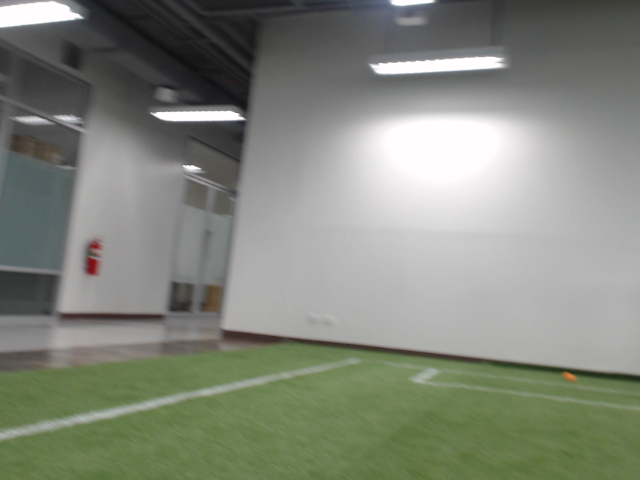
\includegraphics[width=\textwidth]{image/landmark/landmark1.png}
		\end{subfigure}
		\begin{subfigure}{.2\textwidth}
			\centering
			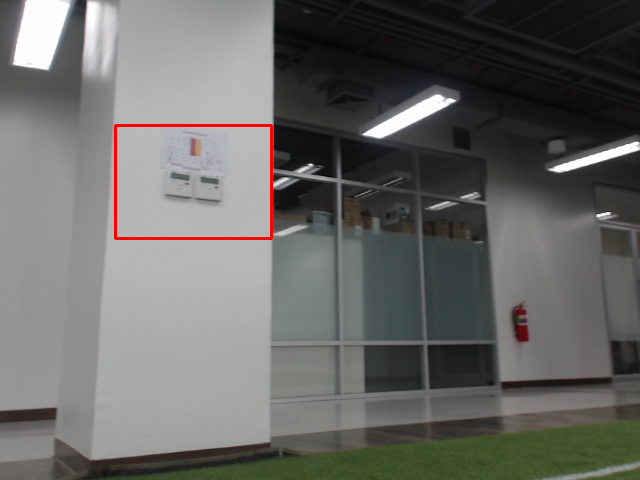
\includegraphics[width=\textwidth]{image/landmark/landmark3.png}
		\end{subfigure}
		\begin{subfigure}{.2\textwidth}
			\centering
			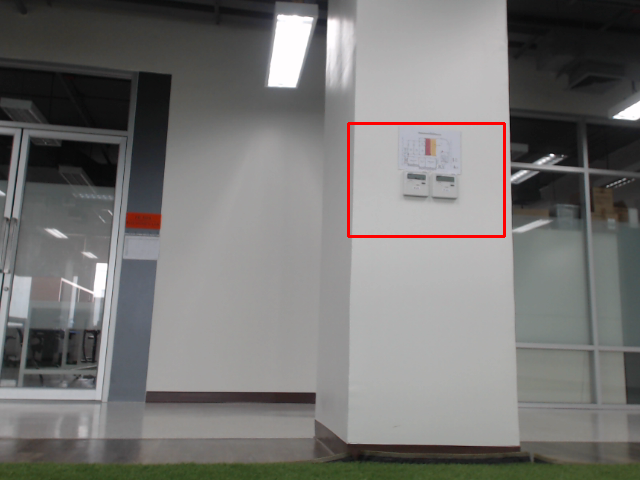
\includegraphics[width=\textwidth]{image/landmark/landmark4.png}
		\end{subfigure}
		\begin{subfigure}{.2\textwidth}
			\centering
			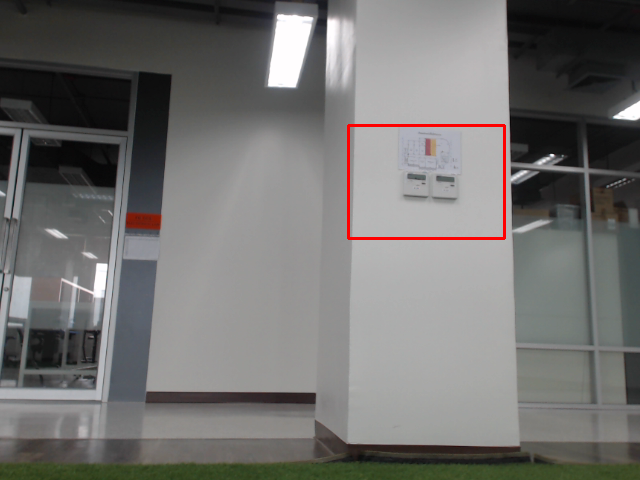
\includegraphics[width=\textwidth]{image/landmark/landmark5.png}
		\end{subfigure}
		\caption{ Demo of landmark tracking with fully-convolution siamese network }
		\label{fig:fig}
	\end{figure}
	
	